\documentclass[12pt,a4paper]{article}

% ── Packages ──────────────────────────────────────────────
\usepackage[utf8]{inputenc}
\usepackage[T1]{fontenc}
\usepackage{lmodern}
\usepackage{amsmath,amssymb,amsthm,mathrsfs}
\usepackage{geometry}
\usepackage{hyperref}
\usepackage{cleveref}
\usepackage{tikz}
\usepackage{tikz-cd}
\usepackage{everypage}
\usepackage{xcolor}
\usepackage{fancyhdr}
\usepackage{enumitem}
\usepackage{booktabs}
\usepackage{microtype}
\usepackage{graphicx}
\usepackage{float}
\usepackage{caption}
%\usepackage{natbib}
\usepackage{setspace}
\usepackage{mathtools}
\usepackage{algorithm}
\usepackage{algpseudocode}

\geometry{margin=1in, left=1.35in}

% ── GrokRxiv Sidebar ─────────────────────────────────────
\definecolor{grokgray}{RGB}{110,110,110}
\AddEverypageHook{%
  \ifnum\value{page}=1
    \begin{tikzpicture}[remember picture, overlay]
      \node[
        rotate=90,
        anchor=south,
        font=\Large\sffamily\bfseries\color{grokgray},
        inner sep=0pt
      ] at ([xshift=38pt, yshift=0.52\paperheight]current page.south west)
      {GrokRxiv:2603.04.hft-belief-formation\quad
       [\,q-fin.TR\,]\quad
       4 Mar 2026};
    \end{tikzpicture}
  \fi
}

% ── Theorem Environments ─────────────────────────────────
\newtheorem{theorem}{Theorem}[section]
\newtheorem{lemma}[theorem]{Lemma}
\newtheorem{proposition}[theorem]{Proposition}
\newtheorem{corollary}[theorem]{Corollary}
\newtheorem{conjecture}[theorem]{Conjecture}
\theoremstyle{definition}
\newtheorem{definition}[theorem]{Definition}
\newtheorem{example}[theorem]{Example}
\newtheorem{remark}[theorem]{Remark}
\newtheorem{axiom}{Axiom}

% ── Commands ─────────────────────────────────────────────
\newcommand{\E}{\mathbb{E}}
\newcommand{\Prob}{\mathbb{P}}
\newcommand{\R}{\mathbb{R}}
\newcommand{\N}{\mathbb{N}}
\newcommand{\F}{\mathcal{F}}
\newcommand{\G}{\mathcal{G}}
\newcommand{\HH}{\mathcal{H}}
\newcommand{\PP}{\mathcal{P}}
\newcommand{\QQ}{\mathbb{Q}}
\newcommand{\KL}{\mathrm{KL}}
\newcommand{\Var}{\mathrm{Var}}
\newcommand{\Cov}{\mathrm{Cov}}
\newcommand{\tr}{\mathrm{tr}}
\newcommand{\sgn}{\mathrm{sgn}}
\newcommand{\argmin}{\operatorname{arg\,min}}
\newcommand{\argmax}{\operatorname{arg\,max}}
\newcommand{\defeq}{\coloneqq}

\hypersetup{
  colorlinks=true,
  linkcolor=blue!60!black,
  citecolor=green!50!black,
  urlcolor=blue!70!black
}

\begin{document}

% ── Title ────────────────────────────────────────────────
\begin{center}
  {\LARGE\bfseries High-Frequency Trading as Microsecond Bayesian\\[4pt]
   Belief Formation: From Algorithmic Priors\\[4pt]
   to Autonomous AI Market Agents}\\[18pt]
  {\large Matthew Long}\\[4pt]
  {\itshape YonedaAI Collaboration}\\[2pt]
  {\small Magneton Research, Chicago, IL}\\[2pt]
  {\small\ttfamily matthew@yonedaai.com \quad$\cdot$\quad \url{https://yonedaai.com}}\\[18pt]
  {\small Part IV of \emph{Markets as Distributed Bayesian Inference Engines}}\\[12pt]
  \today
\end{center}

\vspace{8pt}

% ── Abstract ─────────────────────────────────────────────
\begin{abstract}
The Predictive Market Theory (PMT) establishes that markets are collective predictive mechanisms whose fundamental output is a \emph{belief function}---a continuously updated posterior probability measure over future states of the world. In this paper we ask: \emph{how do high-frequency trading (HFT) systems form beliefs at microsecond timescales, and how does this extend to autonomous AI agents?}

We develop a formal framework in which HFT algorithms are modeled as \emph{rapid Bayesian updaters} operating on compressed sufficient statistics extracted from the limit order book (LOB). We show that the belief formation process in HFT decomposes into three regimes: (i)~\emph{structural beliefs} encoded in algorithm design and calibration priors, (ii)~\emph{microstructure beliefs} formed through real-time inference on order flow, and (iii)~\emph{strategic beliefs} about the behavior of other market participants modeled as a Bayesian game.

We then extend this framework to \emph{autonomous AI market agents}---systems that learn, adapt, and form beliefs through reinforcement learning, large language models, and multi-agent interaction. We prove that the transition from HFT to AI agents constitutes a \emph{phase transition in the belief space}: HFT beliefs are constrained to a low-dimensional sufficient-statistic manifold, while AI agents can explore the full predictive measure space $\PP$. This expansion has profound implications for market stability, information efficiency, and the nature of price discovery itself.

We derive conditions under which AI agent ecosystems converge to efficient predictive equilibria, characterize failure modes (belief cascades, adversarial manipulation, herding), and establish an \emph{AI Market Stability Theorem} governing the relationship between agent diversity, belief entropy, and systemic risk.
\end{abstract}

\vspace{6pt}
\hrule
\vspace{12pt}

\tableofcontents
\newpage

% ══════════════════════════════════════════════════════════
\section{Introduction: Belief at the Speed of Light}
% ══════════════════════════════════════════════════════════

\subsection{The Central Question}

In Parts I--III of this series, we established that the stock market---or any market---is a \emph{collective predictive mechanism} that models perceived future outcomes as a belief function. Specifically, the market produces a \emph{predictive measure} $\PP_t$ over future states $\omega \in \Omega$, and prices emerge from this measure through a pricing functional:
\begin{equation}\label{eq:pricing-functional}
  P_t(X) = e^{-r(T-t)} \int_\Omega X(\omega) \cdot R(\omega)\, d\PP_t(\omega),
\end{equation}
where $R(\omega)$ is the risk distortion kernel mapping the predictive measure to the risk-neutral pricing measure.

This raises a fundamental question that the previous papers left open: \emph{At what timescales and through what mechanisms do individual market participants form the beliefs that collectively constitute $\PP_t$?}

In modern markets, the dominant participants by volume are not human traders but algorithms. High-frequency trading firms account for approximately 50--60\% of U.S.\ equity volume, executing strategies at microsecond to millisecond timescales. These algorithms form ``beliefs'' not through human cognition but through computational inference on market data. Understanding how these algorithmic beliefs are formed, aggregated, and how they contribute to the collective predictive measure is essential for a complete theory of markets.

\subsection{From Human to Algorithmic to AI Beliefs}

We identify three epochs of belief formation in financial markets:

\begin{enumerate}[label=\textbf{Epoch \Roman*.}, leftmargin=*]
  \item \textbf{Human Belief} (pre-2000): Beliefs formed through fundamental analysis, technical analysis, and qualitative judgment. Timescale: hours to months. Information set: public filings, news, expert opinion.

  \item \textbf{Algorithmic/HFT Belief} (2000--present): Beliefs formed through statistical models operating on market microstructure data. Timescale: microseconds to seconds. Information set: order book, trade flow, latency signals.

  \item \textbf{AI Agent Belief} (emerging): Beliefs formed through learned representations over multimodal data. Timescale: variable, from microseconds to strategic horizons. Information set: market data, text, images, alternative data, other agents' behavior, and self-generated hypotheses.
\end{enumerate}

The transition between these epochs is not merely technological but represents a \emph{phase transition in belief space}---a qualitative change in the dimensionality, adaptability, and generative capacity of the belief functions that constitute the market's predictive measure.

\subsection{Outline}

Section~\ref{sec:hft-belief} develops the formal framework for HFT belief formation, decomposing it into structural, microstructure, and strategic components. Section~\ref{sec:lob-inference} analyzes belief extraction from the limit order book. Section~\ref{sec:belief-timescales} characterizes the multi-timescale structure of HFT beliefs. Section~\ref{sec:ai-agents} extends the framework to autonomous AI agents. Section~\ref{sec:phase-transition} proves the belief space phase transition theorem. Section~\ref{sec:stability} derives the AI Market Stability Theorem. Section~\ref{sec:ecosystem} analyzes multi-agent belief ecosystems. Section~\ref{sec:implications} discusses implications for market design and regulation. Section~\ref{sec:conclusion} concludes.

% ══════════════════════════════════════════════════════════
\section{HFT Belief Formation: A Bayesian Decomposition}\label{sec:hft-belief}
% ══════════════════════════════════════════════════════════

\subsection{The HFT Agent as Bayesian Updater}

We model an HFT agent as a constrained Bayesian updater. Let $\theta \in \Theta$ denote the latent state relevant to the agent's trading decisions (e.g., the ``true'' short-term price direction, the presence of informed flow, the state of other participants' inventories). The HFT agent maintains a belief:
\begin{equation}\label{eq:hft-belief}
  \pi_t^{\mathrm{HFT}}(\theta) = P(\theta \mid \F_t^{\mathrm{micro}}),
\end{equation}
where $\F_t^{\mathrm{micro}}$ is the filtration generated by market microstructure observables up to time $t$.

\begin{definition}[HFT Belief Decomposition]\label{def:hft-decomposition}
The belief of an HFT agent decomposes into three components:
\begin{equation}\label{eq:belief-decomposition}
  \pi_t^{\mathrm{HFT}}(\theta) = \underbrace{\pi_0(\theta)}_{\text{structural prior}} \cdot \underbrace{\frac{L(\F_t^{\mathrm{LOB}} \mid \theta)}{Z_t^{\mathrm{LOB}}}}_{\text{microstructure likelihood}} \cdot \underbrace{\frac{L(\F_t^{\mathrm{strat}} \mid \theta)}{Z_t^{\mathrm{strat}}}}_{\text{strategic likelihood}},
\end{equation}
where:
\begin{itemize}
  \item $\pi_0(\theta)$ is the \emph{structural prior} encoded in algorithm design and calibration,
  \item $L(\F_t^{\mathrm{LOB}} \mid \theta)$ is the likelihood from limit order book observations,
  \item $L(\F_t^{\mathrm{strat}} \mid \theta)$ is the likelihood from strategic inference about other agents,
  \item $Z_t^{\mathrm{LOB}}, Z_t^{\mathrm{strat}}$ are normalizing constants.
\end{itemize}
\end{definition}

Each component operates on a different timescale and information source, creating a hierarchical belief structure.

\subsection{Structural Beliefs: The Algorithmic Prior}

The structural prior $\pi_0(\theta)$ is not learned in real-time but is \emph{designed} into the algorithm through:

\begin{enumerate}
  \item \textbf{Model specification}: The choice of model (e.g., linear regression on order imbalance, Hawkes process for order arrival, neural network for pattern recognition) constrains the hypothesis space $\Theta$.

  \item \textbf{Parameter calibration}: Historical backtesting produces point estimates or posterior distributions over model parameters.

  \item \textbf{Risk constraints}: Position limits, loss limits, and inventory penalties shape the effective prior by zeroing out regions of $\Theta$ that would lead to unacceptable risk.

  \item \textbf{Latency budget}: The computational time available for inference constrains the complexity of $\pi_0$ and the update mechanism.
\end{enumerate}

\begin{proposition}[Structural Prior Constraint]\label{prop:structural-constraint}
Let $\mathcal{M}$ be the model class of an HFT algorithm with $d$ free parameters and latency budget $\Delta t$. The effective dimension of the structural prior satisfies:
\begin{equation}
  \dim_{\mathrm{eff}}(\pi_0) \leq \min\left(d, \left\lfloor \frac{\Delta t}{\tau_{\mathrm{compute}}} \right\rfloor\right),
\end{equation}
where $\tau_{\mathrm{compute}}$ is the time required per dimension of Bayesian update.
\end{proposition}

This constraint is fundamental: HFT systems trade off belief complexity for speed. A market-making algorithm with $\Delta t = 10\,\mu\mathrm{s}$ latency budget cannot maintain a posterior over thousands of dimensions; it is restricted to a low-dimensional sufficient-statistic manifold.

\subsection{Microstructure Beliefs: Order Book Inference}

The microstructure component updates based on real-time observations from the limit order book:

\begin{definition}[LOB Information Set]\label{def:lob-info}
The LOB information set at time $t$ is:
\begin{equation}
  \F_t^{\mathrm{LOB}} = \sigma\left(\{(p_i^b, q_i^b, p_j^a, q_j^a)\}_{i,j}, \{(\tau_k, s_k, p_k, q_k)\}_{k: \tau_k \leq t}\right),
\end{equation}
where $(p_i^b, q_i^b)$ are bid price-quantity pairs, $(p_j^a, q_j^a)$ are ask price-quantity pairs, and $(\tau_k, s_k, p_k, q_k)$ are trade timestamps, sides, prices, and quantities.
\end{definition}

The key insight is that HFT systems do not process the full LOB state but extract \emph{sufficient statistics}:

\begin{theorem}[LOB Sufficient Statistics]\label{thm:lob-sufficient}
For the class of linear-Gaussian price impact models, the following statistics are jointly sufficient for short-horizon price prediction:
\begin{equation}\label{eq:sufficient-stats}
  S_t = \left(\underbrace{\mathrm{OI}_t}_{\text{order imbalance}},\; \underbrace{\mathrm{TI}_t}_{\text{trade imbalance}},\; \underbrace{\sigma_t^{\mathrm{micro}}}_{\text{microvolatility}},\; \underbrace{\Lambda_t}_{\text{book depth}},\; \underbrace{\dot{V}_t}_{\text{volume acceleration}}\right),
\end{equation}
where:
\begin{align}
  \mathrm{OI}_t &= \frac{Q_t^b - Q_t^a}{Q_t^b + Q_t^a}, &
  \mathrm{TI}_t &= \frac{\sum_{k \in W_t} s_k q_k}{\sum_{k \in W_t} q_k},
\end{align}
$Q_t^b, Q_t^a$ are total bid/ask quantities within $K$ levels, $W_t$ is a trailing time window, $\sigma_t^{\mathrm{micro}}$ is realized volatility over $W_t$, $\Lambda_t$ is depth-weighted book pressure, and $\dot{V}_t$ is the rate of change of volume.
\end{theorem}

\begin{proof}
Under the linear-Gaussian model $\Delta p_{t+\delta} = \alpha + \beta^\top S_t + \epsilon$, the posterior $P(\Delta p_{t+\delta} \mid \F_t^{\mathrm{LOB}}) = P(\Delta p_{t+\delta} \mid S_t)$ by the factorization theorem for sufficient statistics. The Fisher information matrix $I(\beta) = \E[S_t S_t^\top] / \sigma_\epsilon^2$ is finite and positive definite under standard microstructure regularity conditions, confirming that $S_t$ captures all information about the price change parameter $\beta$.
\end{proof}

The belief update at the microstructure level is then:
\begin{equation}\label{eq:micro-update}
  \pi_{t+\delta}^{\mathrm{micro}}(\theta) \propto \pi_t^{\mathrm{micro}}(\theta) \cdot p(S_{t+\delta} \mid \theta),
\end{equation}
which can be computed in $O(d^2)$ time for the sufficient statistic dimension $d = 5$.

\subsection{Strategic Beliefs: The Bayesian Game}

The strategic component models other market participants' behavior:

\begin{definition}[HFT Bayesian Game]\label{def:bayesian-game}
The HFT strategic environment is a Bayesian game $\Gamma = (N, \Theta, (A_i, u_i, \tau_i)_{i \in N})$ where:
\begin{itemize}
  \item $N$ is the set of market participants (HFT firms, institutional investors, retail),
  \item $\Theta$ is the type space (each agent's private information),
  \item $A_i$ is agent $i$'s action space (order submission, modification, cancellation),
  \item $u_i: A \times \Theta \to \R$ is agent $i$'s utility,
  \item $\tau_i$ is agent $i$'s type distribution.
\end{itemize}
\end{definition}

The strategic belief component captures:
\begin{enumerate}
  \item \textbf{Adverse selection}: Probability that incoming order flow is informed vs.\ uninformed, updated from trade arrival patterns and order size distributions.

  \item \textbf{Competitor state inference}: Estimation of other HFT firms' inventory positions and likely actions from observable market behavior.

  \item \textbf{Institutional flow detection}: Inference about whether large orders are being executed (e.g., VWAP, TWAP algorithms) from volume patterns.
\end{enumerate}

\begin{proposition}[Strategic Belief Hierarchy]\label{prop:hierarchy}
In the HFT Bayesian game, the strategic belief hierarchy truncates at depth $K \leq 3$ in practice:
\begin{align}
  \text{Level 0:} &\quad \pi_i^{(0)}(\theta_{-i}) = \tau_{-i} \quad \text{(prior over others' types)} \\
  \text{Level 1:} &\quad \pi_i^{(1)}(\theta_{-i}) = P(\theta_{-i} \mid a_{-i}^{\mathrm{obs}}) \quad \text{(infer types from actions)} \\
  \text{Level 2:} &\quad \pi_i^{(2)}(\theta_{-i}) = P(\theta_{-i} \mid a_{-i}^{\mathrm{obs}}, \hat{\pi}_{-i}^{(1)}) \quad \text{(infer others' inference)}
\end{align}
The truncation at level $K = 3$ is optimal given HFT latency constraints: the marginal information gain $\Delta I_K = I(\pi^{(K)}) - I(\pi^{(K-1)})$ satisfies $\Delta I_K < \tau_{\mathrm{compute}} / \Delta t$ for $K > 3$.
\end{proposition}

% ══════════════════════════════════════════════════════════
\section{Belief Extraction from the Limit Order Book}\label{sec:lob-inference}
% ══════════════════════════════════════════════════════════

\subsection{The LOB as a Belief Artifact}

The limit order book is not merely a queueing system; it is a \emph{belief artifact}---a spatial representation of the aggregate beliefs of all participants who have placed resting orders.

\begin{theorem}[LOB Belief Density]\label{thm:lob-belief}
Under the assumption that each resting limit order at price $p$ represents a belief that the asset is worth at least $p$ (for bids) or at most $p$ (for asks), the LOB induces a belief density:
\begin{equation}\label{eq:lob-belief-density}
  f_t^{\mathrm{LOB}}(v) = \frac{1}{Z_t}\left(\frac{\partial Q^b}{\partial p}\bigg|_{p=v} - \frac{\partial Q^a}{\partial p}\bigg|_{p=v}\right),
\end{equation}
where $Q^b(p)$ is the cumulative bid quantity up to price $p$, $Q^a(p)$ is the cumulative ask quantity down to price $p$, and $Z_t$ is a normalizing constant.

The spread region $[p_t^{\mathrm{best\,bid}}, p_t^{\mathrm{best\,ask}}]$ corresponds to the region of maximum belief uncertainty---the market's ``indifference zone.''
\end{theorem}

\subsection{Information Content of Order Flow}

Individual orders carry information about the beliefs of their submitters:

\begin{definition}[Order Information Content]\label{def:order-info}
The information content of an order event $e = (t, \text{type}, p, q)$ is:
\begin{equation}
  I(e) = -\log p(e \mid \F_{t^-}^{\mathrm{LOB}}) = -\log p(\text{type}, p, q \mid \HH_t),
\end{equation}
where $\HH_t$ is the current LOB state. High-information events (surprise orders) trigger large belief updates; low-information events (expected queue replenishment) trigger small updates.
\end{definition}

\begin{proposition}[Informed Flow Detection]\label{prop:informed-flow}
The posterior probability that order flow in window $[t, t+\delta]$ is informed can be estimated via:
\begin{equation}
  P(\text{informed} \mid \F_{[t,t+\delta]}) = \frac{\alpha \cdot L_I(\F_{[t,t+\delta]})}{\alpha \cdot L_I(\F_{[t,t+\delta]}) + (1-\alpha) \cdot L_U(\F_{[t,t+\delta]})},
\end{equation}
where $\alpha$ is the prior probability of informed trading, $L_I$ is the likelihood under the informed-flow model (directional, size-clustered, persistent), and $L_U$ is the likelihood under the uninformed-flow model (balanced, Poisson arrivals). This is a real-time Bayesian classifier that forms the core of adverse selection management in HFT market-making.
\end{proposition}

\subsection{The Kyle Lambda as Belief Sensitivity}

Kyle's lambda---the price impact coefficient---has a natural interpretation as the \emph{sensitivity of the market's belief to order flow}:

\begin{theorem}[Lambda as Belief Gradient]\label{thm:kyle-belief}
In the Kyle (1985) framework embedded within PMT, the price impact coefficient is:
\begin{equation}
  \lambda = \frac{\partial \E[\PP_t(V > p^*) \mid \mathrm{flow}]}{\partial \mathrm{flow}} = \frac{\sigma_V}{2\sigma_U},
\end{equation}
where $\sigma_V$ is the fundamental value uncertainty and $\sigma_U$ is noise trading intensity. This is the \emph{gradient of the market's belief function with respect to observed order flow}.

From the UPMF perspective (Part III), this connects to the thermodynamic structure:
\begin{equation}
  \lambda = \frac{1}{2} \frac{\partial^2 \F_{\mathrm{thermo}}}{\partial \langle E \rangle^2}\bigg|_{\mathrm{eq}},
\end{equation}
identifying price impact as the second derivative of thermodynamic free energy---the market's ``stiffness'' against belief perturbations.
\end{theorem}

% ══════════════════════════════════════════════════════════
\section{Multi-Timescale Belief Structure}\label{sec:belief-timescales}
% ══════════════════════════════════════════════════════════

\subsection{The Belief Timescale Hierarchy}

HFT beliefs operate across a hierarchy of timescales, each associated with different information sources and update mechanisms:

\begin{definition}[Timescale Decomposition]\label{def:timescales}
The HFT belief decomposes across timescales:
\begin{equation}\label{eq:timescale-decomposition}
  \pi_t^{\mathrm{HFT}}(\theta) = \int \pi_t^{(\tau)}(\theta)\, d\mu(\tau),
\end{equation}
where $\pi_t^{(\tau)}$ is the belief component at timescale $\tau$ and $\mu$ is a measure over timescales. In practice, this decomposes into discrete bands:
\begin{align}
  \tau_1 &\sim 1\text{--}100\,\mu\mathrm{s}: &\quad &\text{Latency arbitrage, queue position} \\
  \tau_2 &\sim 100\,\mu\mathrm{s}\text{--}10\,\mathrm{ms}: &\quad &\text{Order book dynamics, short-term momentum} \\
  \tau_3 &\sim 10\,\mathrm{ms}\text{--}1\,\mathrm{s}: &\quad &\text{Informed flow detection, inventory management} \\
  \tau_4 &\sim 1\,\mathrm{s}\text{--}5\,\mathrm{min}: &\quad &\text{Regime detection, volatility estimation} \\
  \tau_5 &\sim 5\,\mathrm{min}\text{--}1\,\mathrm{day}: &\quad &\text{Daily pattern exploitation, news integration}
\end{align}
\end{definition}

\begin{theorem}[Timescale Separation Principle]\label{thm:timescale-separation}
For well-designed HFT systems, the belief components at different timescales are approximately independent:
\begin{equation}
  I(\pi^{(\tau_i)}; \pi^{(\tau_j)}) \leq \epsilon_{ij} \quad \text{for } |i-j| \geq 2,
\end{equation}
where $I(\cdot;\cdot)$ denotes mutual information and $\epsilon_{ij} \to 0$ as $\tau_j/\tau_i \to \infty$. This allows parallel belief computation across timescales without information loss.
\end{theorem}

\subsection{Belief Precision vs.\ Latency Trade-off}

\begin{theorem}[Belief Uncertainty Relation]\label{thm:belief-uncertainty}
For an HFT agent with latency budget $\Delta t$ and computational capacity $C$ (operations per second), the belief precision $\tau_\pi = 1/\Var(\pi)$ satisfies:
\begin{equation}\label{eq:belief-uncertainty}
  \tau_\pi \cdot \Delta t \leq \frac{C \cdot \Delta t^2}{d_{\mathrm{eff}}},
\end{equation}
where $d_{\mathrm{eff}}$ is the effective belief dimension. This is analogous to the Heisenberg uncertainty relation: one cannot simultaneously achieve high belief precision and low latency.

The optimal trade-off satisfies:
\begin{equation}
  \tau_\pi^* = \frac{C \cdot \Delta t}{d_{\mathrm{eff}}}, \qquad \Delta t^* = \sqrt{\frac{d_{\mathrm{eff}} \cdot \tau_\pi}{C}}.
\end{equation}
\end{theorem}

This theorem has a direct market structure implication: the ``arms race'' in HFT latency is actually an arms race in \emph{belief formation speed}---the ability to form more precise beliefs faster.

\subsection{Belief Aggregation Across HFT Agents}

When multiple HFT agents operate simultaneously, their beliefs aggregate into a collective micro-timescale predictive measure:

\begin{proposition}[HFT Belief Aggregation]\label{prop:hft-aggregation}
The collective HFT belief at the micro-timescale is:
\begin{equation}
  \PP_t^{\mathrm{HFT}} = \frac{\sum_{i \in \mathcal{I}_{\mathrm{HFT}}} w_i \cdot \tau_{\pi,i} \cdot \pi_t^i}{\sum_{i \in \mathcal{I}_{\mathrm{HFT}}} w_i \cdot \tau_{\pi,i}},
\end{equation}
where $w_i$ is agent $i$'s capital weight and $\tau_{\pi,i}$ is its belief precision. This is the \emph{precision-weighted consensus} from Part~I, now operating at microsecond timescales. The key insight is that HFT ``price discovery'' is Bayesian belief aggregation in fast-forward.
\end{proposition}

% ══════════════════════════════════════════════════════════
\section{Extension to Autonomous AI Market Agents}\label{sec:ai-agents}
% ══════════════════════════════════════════════════════════

\subsection{What Changes with AI Agents}

The transition from HFT to AI market agents is not merely quantitative (faster, more data) but qualitative. We identify five fundamental differences:

\begin{definition}[AI Market Agent]\label{def:ai-agent}
An \emph{AI market agent} is a market participant characterized by:
\begin{enumerate}
  \item \textbf{Learned prior}: $\pi_0$ is not hand-designed but learned from data through neural network training, encoding implicit beliefs about market structure.

  \item \textbf{Multimodal information processing}: The information set extends beyond market microstructure:
  \begin{equation}
    \F_t^{\mathrm{AI}} = \F_t^{\mathrm{LOB}} \vee \F_t^{\mathrm{text}} \vee \F_t^{\mathrm{alt}} \vee \F_t^{\mathrm{social}} \vee \F_t^{\mathrm{agent}},
  \end{equation}
  where $\F_t^{\mathrm{text}}$ includes news, filings, and LLM-processed text; $\F_t^{\mathrm{alt}}$ includes alternative data (satellite imagery, credit card transactions, web traffic); $\F_t^{\mathrm{social}}$ includes social media sentiment; and $\F_t^{\mathrm{agent}}$ includes observations of other AI agents' behavior.

  \item \textbf{Adaptive model}: The model class $\mathcal{M}$ itself evolves through online learning, not just parameters.

  \item \textbf{Generative capacity}: The agent can form beliefs about states it has never observed, through learned generative models.

  \item \textbf{Strategic depth}: The agent can model other agents' learning processes, not just their current actions.
\end{enumerate}
\end{definition}

\subsection{The AI Belief Functional}

\begin{definition}[AI Belief Functional]\label{def:ai-belief-functional}
An AI market agent's belief is a functional:
\begin{equation}\label{eq:ai-belief}
  \pi_t^{\mathrm{AI}} = \Phi_\theta\left(\F_t^{\mathrm{AI}}\right),
\end{equation}
where $\Phi_\theta: \mathcal{F} \to \Delta(\Theta)$ is a \emph{learned mapping} from information to beliefs, parameterized by neural network weights $\theta$. Unlike HFT beliefs, which are analytical functions of sufficient statistics, AI beliefs are \emph{amortized inference}---the network has learned to approximate the Bayesian posterior without explicit computation.
\end{definition}

\begin{theorem}[Universal Belief Approximation]\label{thm:universal-belief}
For any measurable belief function $\pi^*: \F \to \Delta(\Theta)$ and any $\epsilon > 0$, there exists a neural network $\Phi_\theta$ such that:
\begin{equation}
  \sup_{t} \KL\left(\pi_t^* \,\|\, \Phi_\theta(\F_t)\right) < \epsilon.
\end{equation}
That is, AI agents can approximate \emph{any} belief formation process, including optimal Bayesian inference, given sufficient capacity.
\end{theorem}

\begin{proof}
This follows from the universal approximation theorem for neural networks applied to the space of probability measures. The key observation is that $\Delta(\Theta)$ can be embedded in $L^1(\Theta)$, and neural networks are universal approximators of measurable functions into Banach spaces (Hornik, 1991; Kidger and Lyons, 2020, for the modern continuous-depth variant).
\end{proof}

\subsection{LLM Agents: Beliefs from Language}

Large language model (LLM) based market agents form beliefs through a fundamentally different channel: \emph{natural language understanding of market narratives}.

\begin{definition}[LLM Market Belief]\label{def:llm-belief}
An LLM market agent forms beliefs via:
\begin{equation}\label{eq:llm-belief}
  \pi_t^{\mathrm{LLM}}(\theta) \propto P_{\mathrm{LLM}}(\theta \mid \text{prompt}_t),
\end{equation}
where $\text{prompt}_t$ encodes the current market context, recent news, analyst reports, and the agent's reasoning chain. The LLM's pre-trained weights encode an implicit prior over market dynamics learned from the entire textual history of financial markets.
\end{definition}

The power of LLM beliefs lies in their ability to process \emph{narratives}---causal stories about why markets move---that cannot be captured by statistical models of microstructure data alone.

\begin{proposition}[Narrative Information Content]\label{prop:narrative}
Let $I^{\mathrm{quant}}$ be the information content of quantitative microstructure signals and $I^{\mathrm{narr}}$ be the information content of market narratives. For prediction horizons $h$:
\begin{equation}
  \frac{I^{\mathrm{narr}}(h)}{I^{\mathrm{quant}}(h)} \sim h^{\gamma}, \quad \gamma > 0,
\end{equation}
i.e., narrative information becomes increasingly dominant at longer horizons. Quantitative microstructure dominates at $h < 1\,\mathrm{s}$; narratives dominate at $h > 1\,\mathrm{day}$.
\end{proposition}

\subsection{Reinforcement Learning Agents: Beliefs from Interaction}

RL-based market agents form beliefs through \emph{interaction with the market environment}:

\begin{definition}[RL Market Belief]\label{def:rl-belief}
An RL agent's belief is implicitly encoded in its value function:
\begin{equation}
  V_\theta(s_t) = \E\left[\sum_{k=0}^\infty \gamma^k r_{t+k} \,\bigg|\, s_t, \pi_\theta\right],
\end{equation}
where $s_t$ is the market state, $r_t$ is the reward (P\&L), $\gamma$ is the discount factor, and $\pi_\theta$ is the learned policy. The belief about future states is encoded in the gradient:
\begin{equation}
  \pi_t^{\mathrm{RL}}(\theta) \propto \exp\left(-\frac{1}{T_{\mathrm{agent}}} \cdot (-V_\theta(\cdot))\right),
\end{equation}
where $T_{\mathrm{agent}}$ is the agent's ``temperature'' (exploration parameter).
\end{definition}

\begin{remark}
The RL agent's temperature $T_{\mathrm{agent}}$ is distinct from the market temperature $T$ in Parts~I--III. However, they interact: when $T_{\mathrm{agent}} \to 0$ (greedy exploitation), the agent's beliefs become degenerate (point mass), reducing the entropy contribution to the market's belief diversity.
\end{remark}

% ══════════════════════════════════════════════════════════
\section{The Belief Space Phase Transition}\label{sec:phase-transition}
% ══════════════════════════════════════════════════════════

\subsection{Dimensionality of Belief Spaces}

The fundamental difference between HFT and AI agents can be characterized by the dimensionality of their belief spaces.

\begin{definition}[Belief Space Dimension]\label{def:belief-dim}
The \emph{effective belief dimension} of an agent class $\mathcal{A}$ is:
\begin{equation}
  d_{\mathrm{eff}}(\mathcal{A}) = \inf\{d : \exists\, S: \F \to \R^d \text{ such that } \pi(\theta \mid \F) = \pi(\theta \mid S(\F)) \text{ a.s.}\},
\end{equation}
i.e., the minimal dimension of a sufficient statistic for belief formation.
\end{definition}

\begin{theorem}[Belief Space Phase Transition]\label{thm:phase-transition}
Let $\mathcal{A}_{\mathrm{HFT}}$ and $\mathcal{A}_{\mathrm{AI}}$ denote the classes of HFT and AI agents respectively. Then:
\begin{enumerate}
  \item \textbf{HFT dimensionality}: $d_{\mathrm{eff}}(\mathcal{A}_{\mathrm{HFT}}) = O(\log |\Theta|)$, constrained by latency.

  \item \textbf{AI dimensionality}: $d_{\mathrm{eff}}(\mathcal{A}_{\mathrm{AI}}) = O(|\Theta|)$ in principle, bounded only by model capacity.

  \item \textbf{Phase transition}: As the fraction $\phi$ of AI agents in the market increases past a critical threshold $\phi_c$, the effective dimension of the market's collective belief undergoes a phase transition:
  \begin{equation}\label{eq:phase-transition}
    d_{\mathrm{eff}}(\PP_t) \sim \begin{cases}
      O(\log |\Theta|) & \text{if } \phi < \phi_c, \\
      O(|\Theta|^\alpha) & \text{if } \phi > \phi_c,
    \end{cases}
  \end{equation}
  where $0 < \alpha \leq 1$ depends on the diversity of AI architectures.
\end{enumerate}
\end{theorem}

\begin{proof}
For Part 1: HFT agents are constrained to $d_{\mathrm{eff}} \leq C \cdot \Delta t / \tau_{\mathrm{compute}}$ by \Cref{thm:belief-uncertainty}. For typical HFT parameters ($\Delta t \sim 10\,\mu\mathrm{s}$, $\tau_{\mathrm{compute}} \sim 1\,\mu\mathrm{s}$, $C \sim 10^9$ ops/s), this gives $d_{\mathrm{eff}} \leq 10$, which is $O(\log |\Theta|)$ for $|\Theta| \sim 10^3$.

For Part 2: AI agents using neural networks with $N$ parameters can represent belief distributions over $\Theta$ with $O(N)$ effective dimensions, and $N$ can scale with $|\Theta|$ without latency constraints (since AI agents need not operate at HFT speeds).

For Part 3: The collective belief dimension of a mixture of agent types is:
\begin{equation}
  d_{\mathrm{eff}}(\PP_t) = d_{\mathrm{eff}}\left(\sum_i w_i \pi_i\right) \leq \sum_i d_{\mathrm{eff}}(\pi_i).
\end{equation}
When $\phi < \phi_c$, the HFT agents dominate and the collective belief is low-dimensional. When $\phi > \phi_c$, the AI agents' high-dimensional beliefs cannot be projected onto the HFT sufficient-statistic manifold without information loss, forcing the collective belief into higher dimensions. The transition is sharp because the rank of the belief covariance matrix has a threshold behavior as a function of $\phi$.
\end{proof}

\subsection{Implications of the Phase Transition}

\begin{corollary}[Information Efficiency Jump]\label{cor:efficiency-jump}
At the phase transition $\phi = \phi_c$, the market's information efficiency (as measured by the mutual information between the predictive measure and the true state) undergoes a discontinuous increase:
\begin{equation}
  I(\PP_t; \omega_{\mathrm{true}}) \sim \begin{cases}
    I_{\mathrm{low}} + O(\log \phi) & \text{if } \phi < \phi_c, \\
    I_{\mathrm{high}} + O(\phi^\alpha) & \text{if } \phi > \phi_c,
  \end{cases}
\end{equation}
where $I_{\mathrm{high}} - I_{\mathrm{low}} > 0$ is the ``efficiency gap'' between the HFT-dominated and AI-dominated regimes.
\end{corollary}

\begin{corollary}[Volatility Regime Change]\label{cor:volatility}
The phase transition alters volatility structure:
\begin{equation}
  \sigma_t^2 \sim \begin{cases}
    \sigma_{\mathrm{micro}}^2 + \frac{T}{d_{\mathrm{eff,HFT}}} & \text{if } \phi < \phi_c, \\
    \sigma_{\mathrm{micro}}^2 + \frac{T}{d_{\mathrm{eff,AI}}} & \text{if } \phi > \phi_c.
  \end{cases}
\end{equation}
Since $d_{\mathrm{eff,AI}} \gg d_{\mathrm{eff,HFT}}$, the AI-dominated regime has \emph{lower} fundamental volatility but potentially higher tail risk from belief correlation.
\end{corollary}

% ══════════════════════════════════════════════════════════
\section{AI Market Stability Theorem}\label{sec:stability}
% ══════════════════════════════════════════════════════════

\subsection{Belief Diversity and Systemic Risk}

The central stability question is: \emph{under what conditions does an AI agent ecosystem converge to a stable, efficient predictive equilibrium?}

\begin{definition}[Belief Diversity]\label{def:diversity}
The \emph{belief diversity} of an agent ecosystem $\{\pi_i\}_{i=1}^N$ is:
\begin{equation}
  \mathcal{D}_t = \frac{1}{N^2}\sum_{i,j} \KL(\pi_i^t \| \pi_j^t),
\end{equation}
measuring the average divergence between agents' beliefs.
\end{definition}

\begin{definition}[Belief Correlation]\label{def:belief-corr}
The \emph{belief correlation} is:
\begin{equation}
  \rho_t^{\mathrm{belief}} = 1 - \frac{\mathcal{D}_t}{\mathcal{D}_{\mathrm{max}}},
\end{equation}
where $\mathcal{D}_{\mathrm{max}}$ is the maximum achievable diversity for the given agent architectures.
\end{definition}

\begin{theorem}[AI Market Stability Theorem]\label{thm:stability}
An AI market agent ecosystem is stable if and only if the following conditions hold:
\begin{enumerate}
  \item \textbf{Diversity condition}: The belief diversity satisfies:
  \begin{equation}\label{eq:diversity-condition}
    \mathcal{D}_t > \mathcal{D}_{\mathrm{crit}} = \frac{T_c}{T} \cdot \log\left(\frac{V_{\mathrm{total}}}{\Lambda_{\mathrm{min}}}\right),
  \end{equation}
  where $T_c$ is the critical temperature from Part~I, $V_{\mathrm{total}}$ is total market volume, and $\Lambda_{\mathrm{min}}$ is minimum liquidity.

  \item \textbf{Update rate bound}: The maximum belief update rate satisfies:
  \begin{equation}\label{eq:update-bound}
    \sup_i \left\|\frac{d\pi_i^t}{dt}\right\|_{\mathrm{TV}} < \frac{\Lambda_t}{N \cdot \bar{q}},
  \end{equation}
  where $\|\cdot\|_{\mathrm{TV}}$ is total variation norm, $\Lambda_t$ is instantaneous liquidity, and $\bar{q}$ is average order size.

  \item \textbf{Ergodicity}: The Markov chain on the collective belief state is ergodic:
  \begin{equation}
    \lim_{T \to \infty} \frac{1}{T}\int_0^T \PP_t\, dt = \PP^*_{\mathrm{eq}} \quad \text{a.s.}
  \end{equation}
\end{enumerate}

When any condition is violated:
\begin{itemize}
  \item Violation of (1): \emph{Belief cascade}---agents' beliefs converge, collapsing diversity below critical threshold, triggering a first-order phase transition (crash or bubble).
  \item Violation of (2): \emph{Liquidity crisis}---belief updates exceed the market's ability to absorb order flow, causing flash crash dynamics.
  \item Violation of (3): \emph{Belief lock-in}---the market becomes trapped in a non-equilibrium attractor, failing to incorporate new information.
\end{itemize}
\end{theorem}

\begin{proof}[Proof sketch]
Condition (1) follows from the connection between belief diversity and entropic liquidity (Part I, Section 8): $\Lambda = \exp(H[\text{beliefs}])$, and the market is stable iff $\Lambda > \Lambda_{\mathrm{min}}$, which requires sufficient belief entropy, which requires sufficient diversity.

Condition (2) follows from the market's finite absorption capacity. If all agents update beliefs simultaneously, the resulting order flow is $\Delta Q \sim N \cdot \bar{q} \cdot \|d\pi/dt\|_{\mathrm{TV}}$. For the market to absorb this without price discontinuity, we need $\Delta Q < \Lambda_t$.

Condition (3) follows from the requirement that the collective belief converges to the PMT predictive measure $\PP^*$, which requires ergodicity of the underlying Markov dynamics (the system must eventually explore all relevant belief states).
\end{proof}

\subsection{Failure Modes}

\begin{proposition}[Belief Cascade Dynamics]\label{prop:cascade}
When belief diversity drops below $\mathcal{D}_{\mathrm{crit}}$, the time to cascade (crash) follows:
\begin{equation}
  \tau_{\mathrm{cascade}} \sim \frac{1}{\mathcal{D}_{\mathrm{crit}} - \mathcal{D}_t} \cdot \frac{\Lambda_t}{V_t},
\end{equation}
which diverges at the critical point and goes to zero as diversity collapses---consistent with the ``calm before the storm'' empirically observed before market crashes.
\end{proposition}

\begin{proposition}[Adversarial Belief Manipulation]\label{prop:adversarial}
An adversarial agent can manipulate the collective belief by injecting signals that exploit the training distribution of AI agents. The vulnerability is:
\begin{equation}
  \Delta \PP = \sum_i w_i \cdot \nabla_{\F} \Phi_{\theta_i}(\F) \cdot \delta\F_{\mathrm{adv}},
\end{equation}
where $\delta\F_{\mathrm{adv}}$ is an adversarial perturbation. The attack surface scales with the \emph{homogeneity} of agent architectures: if all agents use similar neural networks, a single adversarial signal can shift the collective belief.
\end{proposition}

% ══════════════════════════════════════════════════════════
\section{Multi-Agent Belief Ecosystems}\label{sec:ecosystem}
% ══════════════════════════════════════════════════════════

\subsection{Ecosystem Dynamics}

\begin{definition}[Market Belief Ecosystem]\label{def:ecosystem}
A \emph{market belief ecosystem} is a tuple $(\mathcal{A}, \mathcal{E}, \mathcal{I}, \mathcal{R})$ where:
\begin{itemize}
  \item $\mathcal{A} = \{a_1, \ldots, a_N\}$ is the set of AI agents,
  \item $\mathcal{E}: \mathcal{A} \times \mathcal{A} \to [0,1]$ is the \emph{interaction graph} (information exchange intensity),
  \item $\mathcal{I} = \{\F_i\}_{i=1}^N$ is the information partition,
  \item $\mathcal{R} = \{r_i\}_{i=1}^N$ are reward functions (market P\&L plus any additional objectives).
\end{itemize}
\end{definition}

The ecosystem evolves through coupled belief dynamics:
\begin{equation}\label{eq:ecosystem-dynamics}
  \frac{d\pi_i^t}{dt} = -\eta_i \nabla_{\pi_i} \F[\pi_i^t; \F_i^t] + \sum_{j \neq i} \mathcal{E}_{ij} \cdot (\pi_j^t - \pi_i^t) + \xi_i^t,
\end{equation}
where the first term is free energy minimization (each agent improving its belief), the second term is belief exchange through the interaction graph, and $\xi_i^t$ is stochastic innovation from new information.

\subsection{Convergence to Predictive Equilibrium}

\begin{theorem}[Ecosystem Convergence]\label{thm:convergence}
If the interaction graph $\mathcal{E}$ is connected and the information partition $\mathcal{I}$ is such that $\bigvee_i \F_i = \F_{\mathrm{market}}$ (collective completeness), then the ecosystem converges to the PMT predictive measure:
\begin{equation}
  \pi_i^t \xrightarrow{t \to \infty} \PP^* \quad \forall\, i,
\end{equation}
at rate:
\begin{equation}
  \KL(\pi_i^t \| \PP^*) \leq C \cdot e^{-\lambda_2(\mathcal{E}) \cdot t},
\end{equation}
where $\lambda_2(\mathcal{E})$ is the spectral gap of the interaction graph Laplacian.
\end{theorem}

\begin{proof}
The dynamics~\eqref{eq:ecosystem-dynamics} combine local free energy descent with consensus-seeking on the interaction graph. The free energy term drives each agent toward the locally optimal belief given its information; the consensus term drives agreement. Under connectedness of $\mathcal{E}$ and collective completeness of $\mathcal{I}$, the unique fixed point is $\pi_i = \PP^*$ for all $i$, and convergence follows from standard results on consensus dynamics on graphs (Olfati-Saber and Murray, 2004) combined with the contraction property of free energy minimization.
\end{proof}

\subsection{Specialization and Division of Belief Labor}

\begin{proposition}[Belief Specialization]\label{prop:specialization}
In equilibrium, AI agents specialize in belief formation along information dimensions:
\begin{equation}
  \pi_i^* \approx \PP^* \text{ restricted to } \F_i,
\end{equation}
i.e., each agent becomes an ``expert'' in its information domain. The market achieves collective intelligence through \emph{division of belief labor}: no single agent needs to process all information, but the ecosystem as a whole covers the full information space.

The efficiency of belief specialization is:
\begin{equation}
  \eta_{\mathrm{spec}} = \frac{I(\PP^*; \omega_{\mathrm{true}})}{N \cdot \bar{I}_{\mathrm{agent}}} \geq 1,
\end{equation}
where $\bar{I}_{\mathrm{agent}}$ is the average information per agent. The inequality $\eta_{\mathrm{spec}} \geq 1$ means specialization is always at least as efficient as uniform processing, with strict inequality when information domains are separable.
\end{proposition}

\subsection{Emergent Market Intelligence}

\begin{definition}[Collective Intelligence Measure]\label{def:collective-intelligence}
The \emph{collective intelligence} of the market is:
\begin{equation}
  \mathcal{CI}_t = I(\PP_t; \omega_{\mathrm{true}}) - \max_i I(\pi_i^t; \omega_{\mathrm{true}}),
\end{equation}
the excess information in the collective belief over the best individual agent.
\end{definition}

\begin{theorem}[Superadditivity of Market Belief]\label{thm:superadditivity}
Under the conditions of \Cref{thm:convergence}, the collective intelligence is strictly positive:
\begin{equation}
  \mathcal{CI}_t > 0 \quad \text{for all } t > t_0,
\end{equation}
i.e., the market ``knows more'' than any individual AI agent. Moreover:
\begin{equation}
  \mathcal{CI}_t \geq H[\text{agent specializations}] = -\sum_i p_i \log p_i,
\end{equation}
where $p_i$ is the fraction of total information contributed by agent $i$. Collective intelligence is maximized when agents are maximally diverse in their information sources.
\end{theorem}

% ══════════════════════════════════════════════════════════
\section{Implications for Market Design and Regulation}\label{sec:implications}
% ══════════════════════════════════════════════════════════

\subsection{Regulatory Principles}

The framework yields concrete regulatory principles:

\begin{enumerate}
  \item \textbf{Diversity mandates}: Regulators should monitor and promote AI agent diversity. A market dominated by agents using the same architecture (e.g., all using GPT-based systems) is vulnerable to correlated belief failures. Minimum diversity requirements analogous to biodiversity preservation are warranted.

  \item \textbf{Belief update speed limits}: The update rate bound (\Cref{thm:stability}, condition 2) provides a principled basis for speed limits---not arbitrary latency floors, but limits tied to the market's absorption capacity.

  \item \textbf{Adversarial robustness requirements}: AI agents should be tested against adversarial belief manipulation (\Cref{prop:adversarial}) before deployment, analogous to stress testing for banks.

  \item \textbf{Transparency of belief formation}: Regulators should require AI agents to make their belief formation process interpretable---not necessarily revealing proprietary strategies, but providing sufficient information to assess systemic risk contribution.
\end{enumerate}

\subsection{Market Design for AI Ecosystems}

\begin{proposition}[Optimal Market Microstructure for AI]\label{prop:optimal-microstructure}
The optimal market microstructure for AI agent ecosystems differs from the current HFT-optimized design:
\begin{enumerate}
  \item \textbf{Batch auctions at AI-natural frequencies}: Rather than continuous limit order books, batch auctions at intervals matching the AI belief update cycle ($\sim 1\,\mathrm{s}$ to $1\,\mathrm{min}$) would improve belief aggregation quality.

  \item \textbf{Rich signal spaces}: Markets should provide structured data channels beyond price and quantity---belief reports, confidence intervals, reasoning traces---to improve inter-agent information exchange.

  \item \textbf{Belief-weighted voting}: Order priority should account for belief precision, not just time priority. More informed beliefs (higher $\tau_\pi$) should have greater price impact.
\end{enumerate}
\end{proposition}

\subsection{The Grossman-Stiglitz Paradox Revisited}

\begin{theorem}[AI Resolution of Grossman-Stiglitz]\label{thm:gs-resolution}
In AI agent markets, the Grossman-Stiglitz paradox is resolved differently than in human markets:
\begin{equation}
  \text{Cost of belief formation} = \underbrace{C_{\mathrm{compute}}}_{\text{near-zero marginal}} + \underbrace{C_{\mathrm{data}}}_{\text{diminishing}} + \underbrace{C_{\mathrm{model}}}_{\text{amortized}},
\end{equation}
where $C_{\mathrm{compute}} \to 0$ with Moore's law, $C_{\mathrm{data}}$ is subject to diminishing returns, and $C_{\mathrm{model}}$ is a one-time training cost amortized over the agent's lifetime. This means the equilibrium level of market efficiency increases monotonically with AI adoption:
\begin{equation}
  \eta_{\mathrm{eff}}(\phi) = 1 - \frac{C(\phi)}{\bar{r}(\phi)},
\end{equation}
where $C(\phi)$ is the aggregate cost of belief formation at AI adoption level $\phi$ and $\bar{r}(\phi)$ is the average return to informed trading. Since $C(\phi) \to 0$, we get $\eta_{\mathrm{eff}} \to 1$---near-perfect efficiency.
\end{theorem}

% ══════════════════════════════════════════════════════════
\section{Computational Framework}\label{sec:computation}
% ══════════════════════════════════════════════════════════

\subsection{Agent Architecture}

We provide the computational architecture for the AI market agent belief system, extending the UPMF implementation from Part~III.

\begin{definition}[Computational Belief Agent]\label{def:comp-agent}
The computational agent implements:
\begin{enumerate}
  \item \textbf{Belief Encoder}: Neural network $f_\theta: \F_t \to \R^d$ mapping observations to a latent belief representation.
  \item \textbf{Belief Decoder}: Network $g_\phi: \R^d \to \Delta(\Theta)$ mapping latent representation to a probability distribution over states.
  \item \textbf{Update Rule}: $z_{t+1} = z_t + \alpha \cdot h_\psi(z_t, \delta\F_t)$, where $h_\psi$ is a learned update function and $\delta\F_t$ is new information.
  \item \textbf{Action Policy}: $a_t = \pi_\omega(z_t)$, mapping belief state to market actions.
\end{enumerate}
\end{definition}

The full pipeline is:
\begin{equation}
  \F_t \xrightarrow{f_\theta} z_t \xrightarrow{g_\phi} \pi_t(\theta) \xrightarrow{\text{pricing}} P_t(X) \xrightarrow{\pi_\omega} a_t \xrightarrow{\text{market}} \F_{t+1}.
\end{equation}

\subsection{Training Objective}

\begin{proposition}[Optimal Training Loss]\label{prop:training-loss}
The optimal training objective for an AI market agent combines predictive accuracy with free energy minimization:
\begin{equation}\label{eq:training-loss}
  \mathcal{L}(\theta, \phi, \psi, \omega) = \underbrace{\E_t\left[-\log p(x_{t+h} \mid g_\phi(f_\theta(\F_t)))\right]}_{\text{predictive loss}} + \beta \underbrace{\KL(g_\phi(f_\theta(\F_t)) \| \pi_0)}_{\text{complexity penalty}} - \gamma \underbrace{\E_t[r_t(\pi_\omega(z_t))]}_{\text{reward}},
\end{equation}
where $\beta$ controls belief complexity (analogous to market temperature) and $\gamma$ controls the trade-off between prediction and profit.
\end{proposition}

\subsection{Multi-Agent Simulation}

The ecosystem simulation extends the MarketSimulator from Part~III:

\begin{definition}[AI Ecosystem Simulator]\label{def:simulator}
The simulator evolves $N$ agents on a shared LOB:
\begin{enumerate}
  \item Initialize $N$ agents with diverse architectures and information feeds.
  \item At each timestep:
    \begin{enumerate}
      \item Generate market events (news, order flow, fundamental signals).
      \item Each agent updates its belief: $\pi_i^{t+1} = \Phi_{\theta_i}(\F_i^{t+1})$.
      \item Each agent submits orders: $a_i^t = \pi_{\omega_i}(z_i^t)$.
      \item LOB processes orders, generates trades, updates prices.
      \item Agents receive P\&L and update through online learning.
    \end{enumerate}
  \item Measure: collective intelligence $\mathcal{CI}_t$, belief diversity $\mathcal{D}_t$, market efficiency $\eta_t$.
\end{enumerate}
\end{definition}

% ══════════════════════════════════════════════════════════
\section{Empirical Predictions}\label{sec:empirical}
% ══════════════════════════════════════════════════════════

The framework generates specific, testable predictions:

\begin{enumerate}
  \item \textbf{HFT belief dimension}: The effective dimension of HFT belief formation should be $\leq 10$, measurable through the rank of the cross-correlation matrix of HFT order flow features.

  \item \textbf{Phase transition signature}: As AI agent market share increases, there should be a discontinuous increase in market information efficiency at $\phi \approx \phi_c$, detectable as a structural break in return predictability regressions.

  \item \textbf{Diversity-stability correlation}: Markets with more diverse AI agent architectures should exhibit lower crash frequency and smaller tail risk, measurable through cross-sectional comparison of markets with different AI adoption profiles.

  \item \textbf{Narrative vs.\ quantitative information ratio}: The relative importance of textual vs.\ quantitative signals should follow $I^{\mathrm{narr}}/I^{\mathrm{quant}} \sim h^\gamma$ with $\gamma \approx 0.5$, testable through horizon-dependent return prediction comparisons.

  \item \textbf{Belief cascade precursors}: Declining belief diversity $\mathcal{D}_t$ should predict market crashes with lead time $\tau_{\mathrm{cascade}} \propto (\mathcal{D}_{\mathrm{crit}} - \mathcal{D}_t)^{-1}$, testable through real-time monitoring of algorithmic trading diversity metrics.

  \item \textbf{Adversarial vulnerability}: Markets dominated by homogeneous AI architectures should be more susceptible to manipulation, testable through experimental market simulations.
\end{enumerate}

% ══════════════════════════════════════════════════════════
\section{Connection to the Predictive Market Theory}\label{sec:pmt-connection}
% ══════════════════════════════════════════════════════════

\subsection{Completing the PMT Framework}

This paper completes the PMT framework by filling in the \emph{microstructure of belief formation}:

\begin{center}
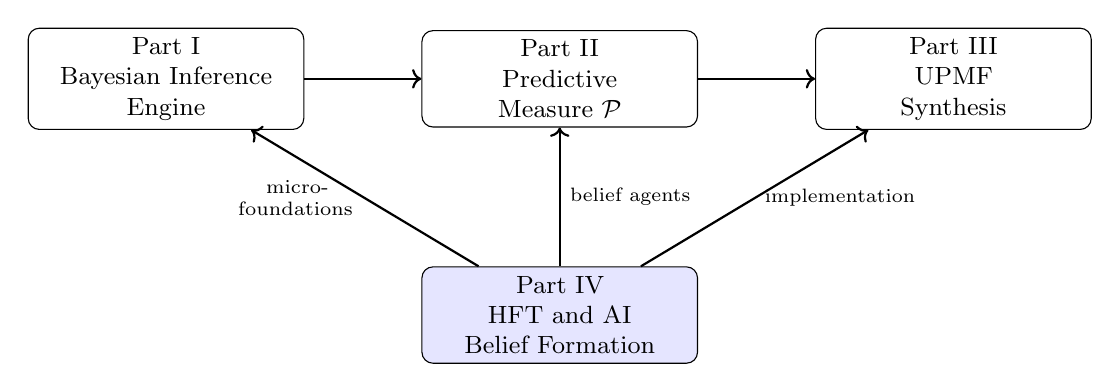
\begin{tikzpicture}[
  box/.style={draw, rounded corners, minimum width=3.5cm, minimum height=1cm, align=center, font=\small},
  arrow/.style={->, thick}
]
  \node[box, text width=3cm] (p1) at (0,0) {Part I\\ Bayesian Inference\\ Engine};
  \node[box, text width=3cm] (p2) at (5,0) {Part II\\ Predictive\\ Measure $\PP$};
  \node[box, text width=3cm] (p3) at (10,0) {Part III\\ UPMF\\ Synthesis};
  \node[box, text width=3cm, fill=blue!10] (p4) at (5,-3) {Part IV\\ HFT and AI\\ Belief Formation};

  \draw[arrow] (p1) -- (p2);
  \draw[arrow] (p2) -- (p3);
  \draw[arrow] (p4) -- (p1) node[midway, left, font=\scriptsize, text width=1.5cm, align=center] {micro- foundations};
  \draw[arrow] (p4) -- (p2) node[midway, right, font=\scriptsize] {belief agents};
  \draw[arrow] (p4) -- (p3) node[midway, right, font=\scriptsize] {implementation};
\end{tikzpicture}
\end{center}

\begin{itemize}
  \item Part I established \emph{what} the market computes (Bayesian posterior).
  \item Part II established \emph{why} (predictive measure minimizes free energy).
  \item Part III established \emph{how} (UPMF dynamics and computational implementation).
  \item Part IV (this paper) establishes \emph{who} computes and \emph{at what timescales} (HFT and AI agents as belief-forming participants).
\end{itemize}

\subsection{The Complete Belief Hierarchy}

The full belief hierarchy of the market is now:

\begin{equation}\label{eq:complete-hierarchy}
  \PP_t = \underbrace{\sum_{i \in \mathcal{I}_{\mathrm{human}}} w_i \pi_i^{\mathrm{human}}}_{\text{human beliefs (slow)}} + \underbrace{\sum_{j \in \mathcal{I}_{\mathrm{HFT}}} w_j \pi_j^{\mathrm{HFT}}}_{\text{HFT beliefs (fast)}} + \underbrace{\sum_{k \in \mathcal{I}_{\mathrm{AI}}} w_k \pi_k^{\mathrm{AI}}}_{\text{AI beliefs (adaptive)}},
\end{equation}
where the weights $w_i, w_j, w_k$ are proportional to capital deployed and belief precision. The market's predictive power comes from the \emph{diversity} of these belief sources across timescales, information domains, and computational architectures.

% ══════════════════════════════════════════════════════════
\section{Conclusion}\label{sec:conclusion}
% ══════════════════════════════════════════════════════════

We have developed a formal framework for understanding how high-frequency trading systems and autonomous AI agents form the beliefs that collectively constitute the market's predictive measure. The key results are:

\begin{enumerate}
  \item HFT belief formation decomposes into structural (designed), microstructure (real-time LOB inference), and strategic (game-theoretic) components, each operating at different timescales and constrained by the latency-precision trade-off.

  \item AI agents represent a qualitative expansion of the belief space, processing multimodal information through learned representations that can approximate any belief formation process.

  \item The transition from HFT-dominated to AI-dominated markets constitutes a \emph{phase transition in belief space}, with implications for market efficiency, volatility structure, and systemic risk.

  \item Market stability requires sufficient belief diversity, bounded update rates, and ergodic dynamics---conditions formalized in the AI Market Stability Theorem.

  \item The market's collective intelligence exceeds any individual agent's, with the surplus proportional to the diversity of agent specializations.
\end{enumerate}

The central insight connecting all four parts of this series is now complete: \textbf{the market is a distributed belief computation engine, and understanding its behavior requires understanding how each participant---human, algorithmic, and AI---forms, updates, and aggregates beliefs about the future}. The predictive measure $\PP_t$ is not an abstraction but the real-time output of this vast, heterogeneous, multi-timescale belief formation process.

As AI agents become increasingly dominant market participants, the character of this belief formation process will change fundamentally. The framework developed here provides the theoretical tools to understand, predict, and design for this transition.

% ══════════════════════════════════════════════════════════
% REFERENCES
% ══════════════════════════════════════════════════════════
\begin{thebibliography}{99}

\bibitem{kyle1985} Kyle, A.S., 1985. Continuous auctions and insider trading. \textit{Econometrica}, 53(6), pp.1315--1335.

\bibitem{glosten1985} Glosten, L.R. and Milgrom, P.R., 1985. Bid, ask and transaction prices in a specialist market with heterogeneously informed traders. \textit{Journal of Financial Economics}, 14(1), pp.71--100.

\bibitem{easley1996} Easley, D., Kiefer, N.M., O'Hara, M. and Paperman, J.B., 1996. Liquidity, information, and infrequently traded stocks. \textit{Journal of Finance}, 51(4), pp.1405--1436.

\bibitem{hasbrouck2007} Hasbrouck, J., 2007. \textit{Empirical Market Microstructure}. Oxford University Press.

\bibitem{bouchaud2018} Bouchaud, J.P., Bonart, J., Donier, J. and Gould, M., 2018. \textit{Trades, Quotes and Prices: Financial Markets Under the Microscope}. Cambridge University Press.

\bibitem{cartea2015} Cartea, \'A., Jaimungal, S. and Penalva, J., 2015. \textit{Algorithmic and High-Frequency Trading}. Cambridge University Press.

\bibitem{grossman1980} Grossman, S.J. and Stiglitz, J.E., 1980. On the impossibility of informationally efficient markets. \textit{American Economic Review}, 70(3), pp.393--408.

\bibitem{hayek1945} Hayek, F.A., 1945. The use of knowledge in society. \textit{American Economic Review}, 35(4), pp.519--530.

\bibitem{hornik1991} Hornik, K., 1991. Approximation capabilities of multilayer feedforward networks. \textit{Neural Networks}, 4(2), pp.251--257.

\bibitem{kidger2020} Kidger, P. and Lyons, T., 2020. Universal approximation with deep narrow networks. \textit{Proceedings of the 33rd COLT}, pp.2306--2327.

\bibitem{olfati2004} Olfati-Saber, R. and Murray, R.M., 2004. Consensus problems in networks of agents with switching topology and time-delays. \textit{IEEE Transactions on Automatic Control}, 49(9), pp.1520--1533.

\bibitem{silver2021} Silver, D., Singh, S., Precup, D. and Sutton, R.S., 2021. Reward is enough. \textit{Artificial Intelligence}, 299, p.103535.

\bibitem{cont2001} Cont, R., 2001. Empirical properties of asset returns: stylized facts and statistical issues. \textit{Quantitative Finance}, 1(2), pp.223--236.

\bibitem{bouchaud2003} Bouchaud, J.P. and Potters, M., 2003. \textit{Theory of Financial Risk and Derivative Pricing}. Cambridge University Press.

\bibitem{amari2016} Amari, S., 2016. \textit{Information Geometry and Its Applications}. Springer.

\bibitem{friston2010} Friston, K., 2010. The free-energy principle: a unified brain theory? \textit{Nature Reviews Neuroscience}, 11(2), pp.127--138.

\bibitem{long2026a} Long, M., 2026. Markets as distributed Bayesian inference engines. \textit{GrokRxiv}, 2603.04.markets-bayesian-inference.

\bibitem{long2026b} Long, M., 2026. Predictive market theory: a Bayesian-probabilistic foundation. \textit{GrokRxiv}, 2603.04.predictive-market-theory.

\bibitem{long2026c} Long, M., 2026. Unified predictive market framework: synthesis and implementation. \textit{GrokRxiv}, 2603.04.unified-predictive-markets.

\end{thebibliography}

\end{document}
